 \section{Design of CUDA Kernels}
 \label{2017-lu-block-jacobi:sec:kernel}

This section describes the implementation
of efficient CUDA kernels for both batched LU factorization
as well as triangular system solves
specifically tuned for small problem sizes
where the system matrix (corresponding to a diagonal block in block-Jacobi preconditioning) 
contains at most $32 \times 32$ elements.
This is consistent with the batched implementation of GH in~\cite{gh}
which is also designed for small problems, of the type arising in block-Jacobi preconditioning.

\begin{figure}[t]
\begin{center}
\begin{minipage}{0.9\columnwidth}
{\small
\lstinputlisting[language=matlab,caption=,morekeywords={SpMV,ddot,daxpy,dscal}]{code/LU.m}
}
\end{minipage}
\begin{minipage}{0.9\columnwidth}
{\small
\lstinputlisting[language=matlab,caption=,morekeywords={SpMV,ddot,daxpy,dscal}]{code/LUI.m}
}
\end{minipage}
\caption
[Basic LU factorization in Matlab notation using explicit and implicit pivoting]
{Loop-body of the basic LU factorization in Matlab notation
    using explicit and implicit partial pivoting (top and bottom, respectively).}
\label{2017-lu-block-jacobi:fig:lu}
\end{center}
\end{figure}

\begin{figure}[t]
\begin{center}
\begin{tabular}{c}
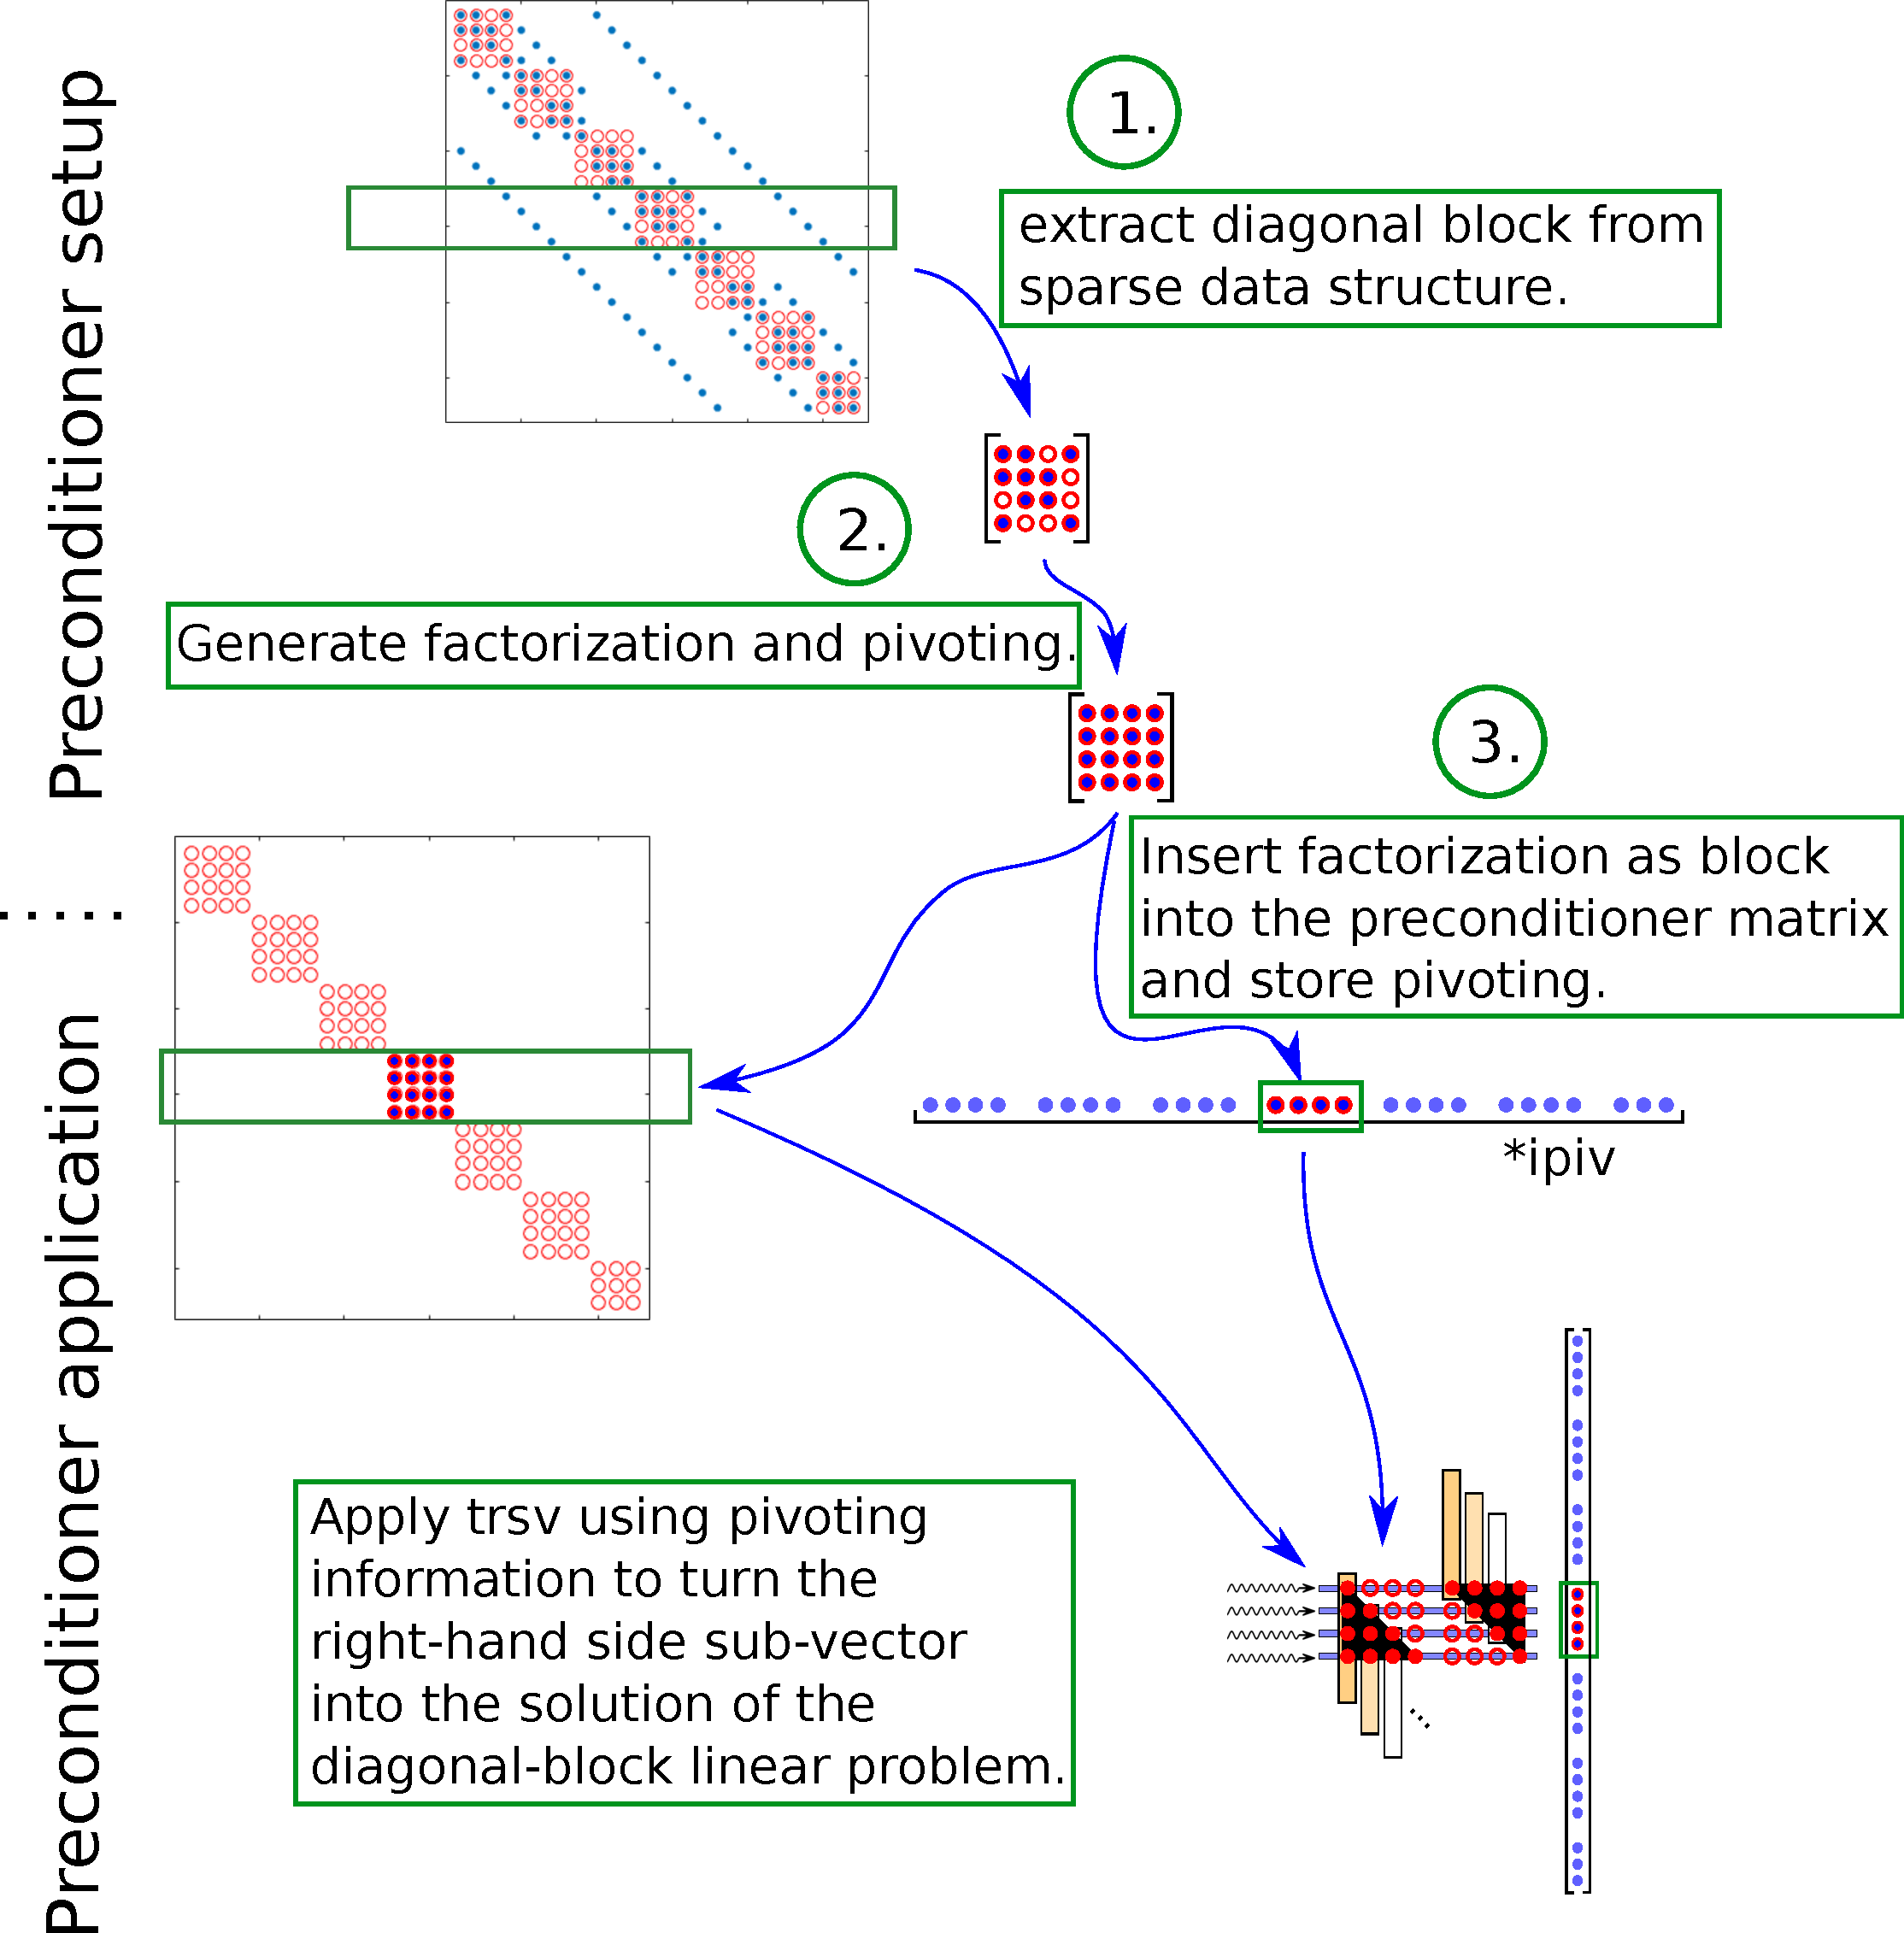
\includegraphics[width=.6\columnwidth]{plots/fact_based_blockJacobi}
\end{tabular}
\end{center}
\caption
[Batched factorization and triangular solve ({\sc trsv}) 
in a block-Jacobi preconditioner setting]
{Using batched factorization and batched triangular solve ({\sc trsv}) 
         routines in a block-Jacobi preconditioner setting.%
}
\label{2017-lu-block-jacobi:fig:precscheme}
\end{figure}

\subsection{Batched LU factorization ({\sc getrf})}

A simplified MATLAB routine for the
(right-looking) LU factorization of a square block \texttt{Di} is shown in Figure~\ref{2017-lu-block-jacobi:fig:lu} (top).
This algorithmic variant lies in the foundations of our batched CUDA kernel for this factorization that
we discuss next.

Recent GPU architectures from NVIDIA 
feature a large amount of registers per thread
which makes it possible to assign problems of size up to $32 \times 32$
to a single warp.
Each thread then stores one row of the system matrix \texttt{Di}
into the local registers,
while warp shuffle instructions
allow to access elements from other rows
(e.g., when performing the updates in lines 13--15).
Using this technique, it is possible to read the system matrix only once,
and perform the whole factorization process in the registers,
avoiding the latency of memory and caches,
as well as additional load and store instructions.

A complementary optimization, also important,
addresses the pivoting procedure ensuring the practical stability of the LU factorization.
Even though the selection of the pivot row \texttt{ipiv} (lines 6--7)
in step \texttt{k} of the factorization
can be realized efficiently using a parallel reduction,
the actual exchange of rows \texttt{k} and \texttt{ipiv} (lines 8--9) on a GPU is costly,
as it involves only the two threads holding these rows,
while the remaining threads stay idle.
To tackle this issue, in~\cite{gje,gh} 
we proposed an implicit pivoting procedure
for GJE and GH, which avoids the explicit row swaps and combines them into
a single, easily parallelizable permutation,
which is performed after the main loop.
This technique can also be applied to LU by observing the following:
\begin{itemize}
\item During step \texttt{k} of the factorization,
    the operation performed on each row of the matrix (lines 13--15)
    depends only on the elements in this row and the pivot row \texttt{ipiv}
    (which was exchanged with row \texttt{k}
    when using standard, explicit pivoting as in Figure~\ref{2017-lu-block-jacobi:fig:lu}).
\item The type of operation to perform on each row
    can be derived without knowing its position in the matrix:
    if the row has already been pivoted, then no operation is required
    (in Figure~\ref{2017-lu-block-jacobi:fig:lu} such row was exchanged
    with one of the first \texttt{k} rows);
    otherwise the \texttt{k}-th element of the row has to be scaled
    (line 13),
    and an {\sc axpy} needs to be performed on the trailing vector (lines 14--15).
\end{itemize}
These observations turn the implicit pivoting procedure for LU
even more efficient than its counterpart applied in GH,
as the operations performed by each thread
do not depend on the previously selected pivot rows.
Conversely, for GH a list of their indices
has to be replicated in each thread~\cite{gh}.
As an illustration, the bottom factorization code in Figure~\ref{2017-lu-block-jacobi:fig:lu}
shows the implicit pivoting approach in the LU factorization.
A final optimization can be made by combining the row swap
with the off-load of $L$ and $U$ to main memory,
hereby eliminating all inter-thread communication induced by row swaps.
In addition to writing the triangular factors,
the pivoting information also has to
be stored in main memory for the subsequent triangular solves,
see Figure~\ref{2017-lu-block-jacobi:fig:precscheme}.

\begin{figure}[t]
\begin{center}
\begin{tabular}{c}
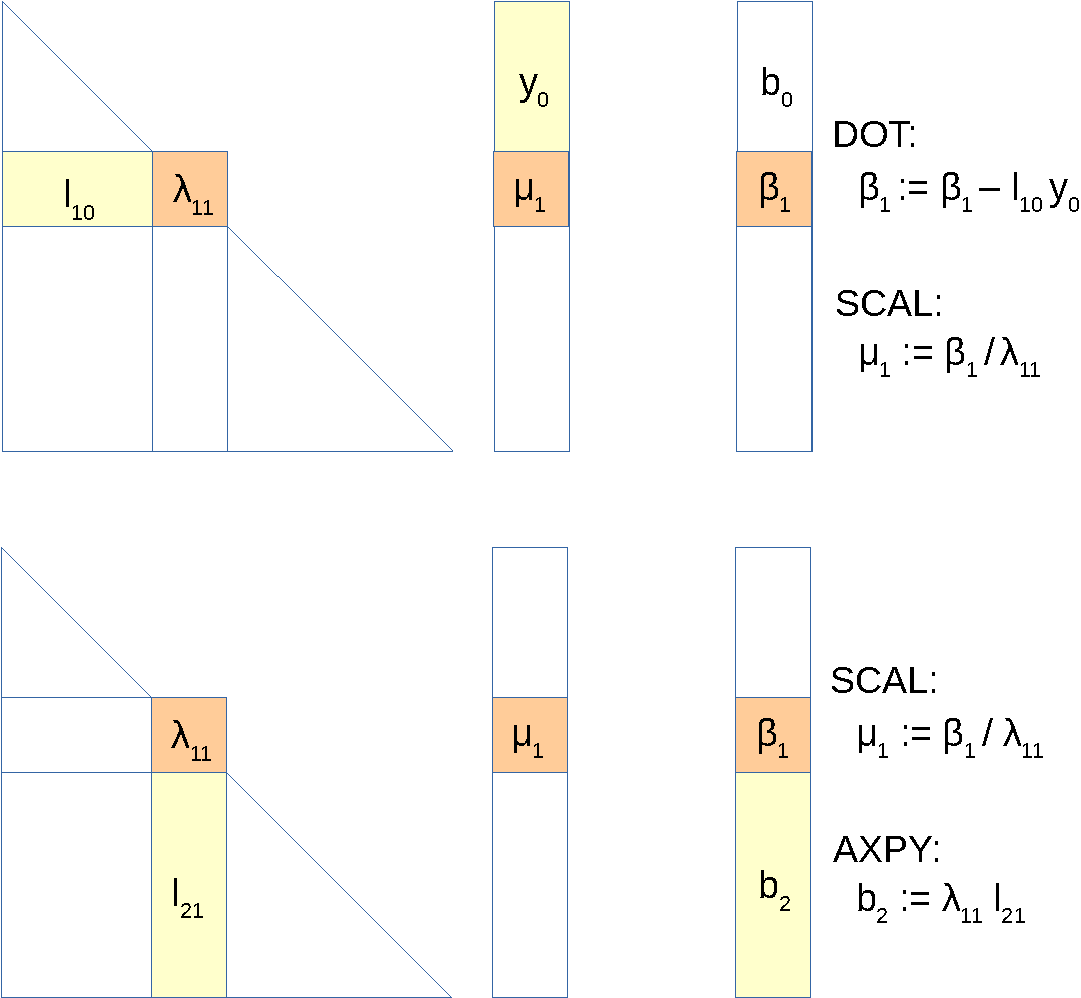
\includegraphics[width=.5\columnwidth]{plots/lazy_eagar}
\end{tabular}
\end{center}
\caption
[Illustration of the ``lazy'' and ``eager'' \textsc{trsv} algorithms variants]
{Illustration of the ``lazy'' and ``eager'' algorithmic variants (top and bottom, respectively)
    for the solution of a unit lower triangular system.}
\label{2017-lu-block-jacobi:fig:trsfig}
\end{figure}


\begin{figure}[t]
\begin{center}
\begin{minipage}{0.9\columnwidth}
{\small
\lstinputlisting[language=matlab,caption=,morekeywords={SpMV,ddot,daxpy,dscal}]{code/TRS_L.m}
}
\end{minipage}
\begin{minipage}{0.9\columnwidth}
{\small
\lstinputlisting[language=matlab,caption=,morekeywords={SpMV,ddot,daxpy,dscal}]{code/TRS_E.m}
}
\end{minipage}
\caption
[Loop-body of the ``lazy'' and ``eager'' \textsc{trsv} algorithms variants]
{Loop-body of the ``lazy'' and ``eager'' algorithmic variants (top and bottom, respectively)
for the solution of a unit lower triangular system in Matlab notation.}
\label{2017-lu-block-jacobi:fig:trs}
\end{center}
\end{figure}

\begin{figure}[p]
\begin{center}
\begin{tabular}{c}
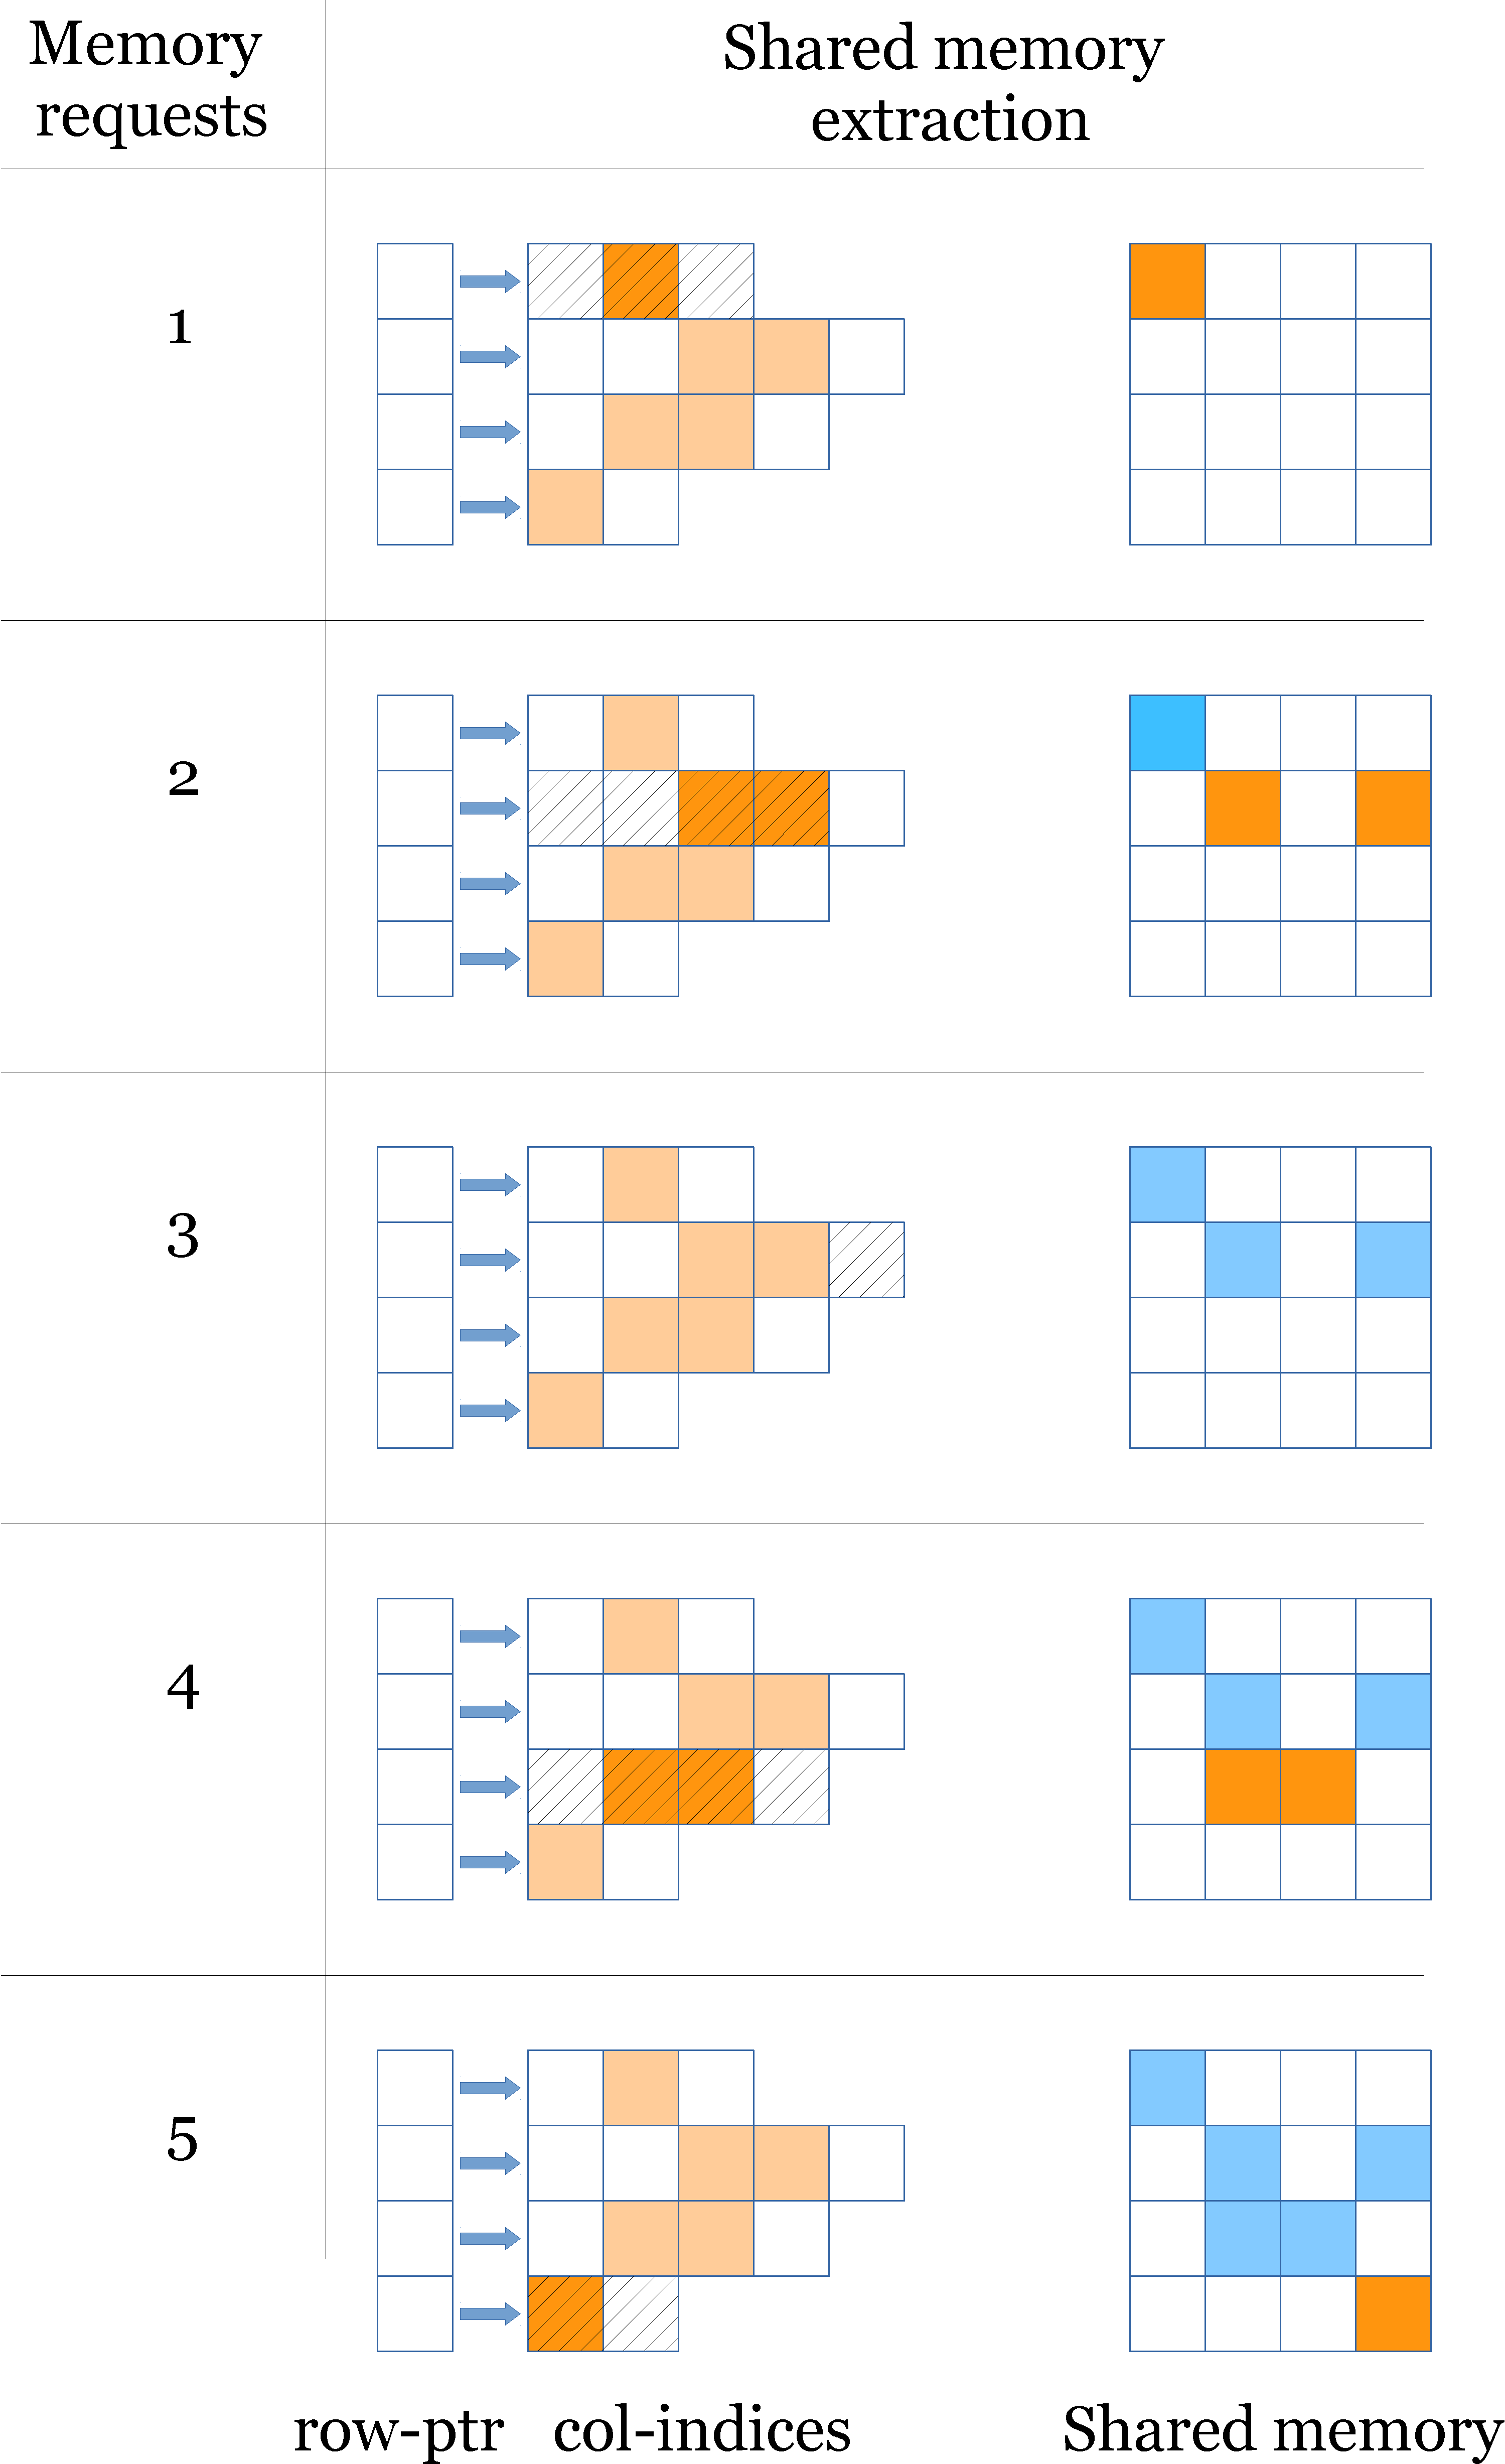
\includegraphics[width=.5\columnwidth]{plots/extraction}
\end{tabular}
\end{center}
\caption
[Illustration of the memory requests for the shared memory extraction]
{Illustration of the memory requests for the shared memory extraction.
The elements part of the diagonal block are colored in light orange, the elements that have already been extracted in light blue.
We assume warps of 4 threads, and visualize the data read by the distinct threads at each iteration with dashed cells.
If an element part of the diagonal block is currently accessed (dark orange) it is extracted and stored in the correct location
in shared memory (dark orange also in the shared memory).
We only show the accesses to the vector storing the {\sf col-indices} of the CSR matrix structure~\cite{saad}; 
the access to the actual values induces far less overhead,
as these memory locations are accessed only if a location belonging to a diagonal block is found.
In that case, the access pattern is equivalent to the one used for {\sf col-indices}.
}
\label{2017-lu-block-jacobi:fig:extraction}
\end{figure}

\subsection{Batched triangular system solves ({\sc trsv})}

Unlike the LU factorization,
the triangular system solves offer only a limited amount of data reuse.
Each element of the triangular factors is needed only once,
so explicitly keeping this value in registers does not offer any advantage.
In contrast, the right-hand side vector $b$, which is overwritten with the solution 
vector, is reused.
Hence, it is beneficial to read and distribute this vector across the registers
of the threads in the warp (one element per thread).

The permutation $b := Pb$ coming from pivoting
is performed while reading $b$ into the registers:
Each element is stored to the registers of the correct threads.
This step is followed by a unit lower triangular solve, and finally an upper triangular solve.
As these operations are similar, we will for brevity only discuss 
the lower triangular solve (the solution of $Ly = b (= Pb)$) in detail.
There exist different strategies for realizing the triangular solve:
the ``lazy'' variant (Figure~\ref{2017-lu-block-jacobi:fig:trsfig} and the code in Figure~\ref{2017-lu-block-jacobi:fig:trs}, top) relies on an inner ({\sc dot}) product
to compute the final value of $y_k$ at step \texttt{k},
while the ``eager'' one (Figure~\ref{2017-lu-block-jacobi:fig:trsfig} and the code in Figure~\ref{2017-lu-block-jacobi:fig:trs}, bottom) leverages an {\sc axpy}
to update the trailing vector $y_{k+1:m}$.
In this case the latter variant is more convenient,
as the parallelization of {\sc axpy} is straightforward,
while the {\sc dot} product requires a reduction.
The memory accesses to the system matrix are also different:
the ``lazy'' variant reads one row per step,
while the ``eager'' one reads one column.
Therefore, assuming standard column-major storage,
the ``eager'' variant also has the benefit of coalesced memory access.

\subsection{Block-Jacobi preconditioning using batched LU}
Using batched factorization routines for block-Jacobi preconditioning
requires the extraction of the diagonal blocks from the sparse system matrix. 
This is a non-trivial step as accessing a (dense) diagonal block embedded in a 
sparse data structure (such as those typically used for storing the system matrix, e.g., CSR~\cite{saad})
can be quite elaborate. Furthermore, exploiting the fine-grained parallelism
provided by the GPU hardware in the extraction step makes this operation
challenging for problems with an unbalanced sparsity pattern:
Assigning the parallel resources to the distinct rows will inevitably result in severe
work imbalance for problems with a very unbalanced nonzero distribution, 
like for example those arising in circuit simulation.
Additionally, accessing the distinct rows in the row-major-based CSR layout in parallel
results in non-coalescent data access.
In~\cite{gje} we proposed a strategy to overcome the latter drawback while 
simultaneously diminishing the effects of the former one by means of 
an intermediate step which stores the diagonal blocks in shared memory.
Although we refrain 
from showing a comparison between the standard approach and the shared memory based
strategy in the experimental section, we recall the central ideas of this \textit{shared memory extraction} 
for convenience:


Instead of assigning the distinct threads within the warp to the distinct rows
corresponding to the diagonal block,
all threads of the warp collaborate to process each row.
The threads accessing an element that is part of the diagonal block extract the respective value
and store it into shared memory. This allows for coalescent access to the elements 
stored in CSR format, and avoids the load imbalance up to a level where load imbalance 
only occurs between threads of the same warp.
After extracting the elements that are part of the diagonal block,
they are copied into registers of the thread
that will handle the respective row in the factorization process.
Figure~\ref{2017-lu-block-jacobi:fig:extraction} visualizes this
diagonal block extraction strategy~\cite{gje}.


